\section{CSP}
Represent problems as constraint graphs; nodes are variables, edges are constraints. Can solve with backtracking search (DFS, try assigning variables until you run into a contradiction, backtrack, can be implemented recursively), forward checking (when a variable is assigned, check consistency of all arcs from unassigned variables to newly assigned variable), arc constistency (if a variable $X$ loses a value in its domain of possible values when checking arc consistency, check all of its neighbors). An arc from unassigned $X$ to assigned $Y$ (i.e. $X\rightarrow Y$) is consistent iff for every $x\in X$, there is some $y\in Y$ which could be assigned without violating a constraint; when checking consistency, delete invalid assignments from $X$.
\begin{figure}[H]
\centering
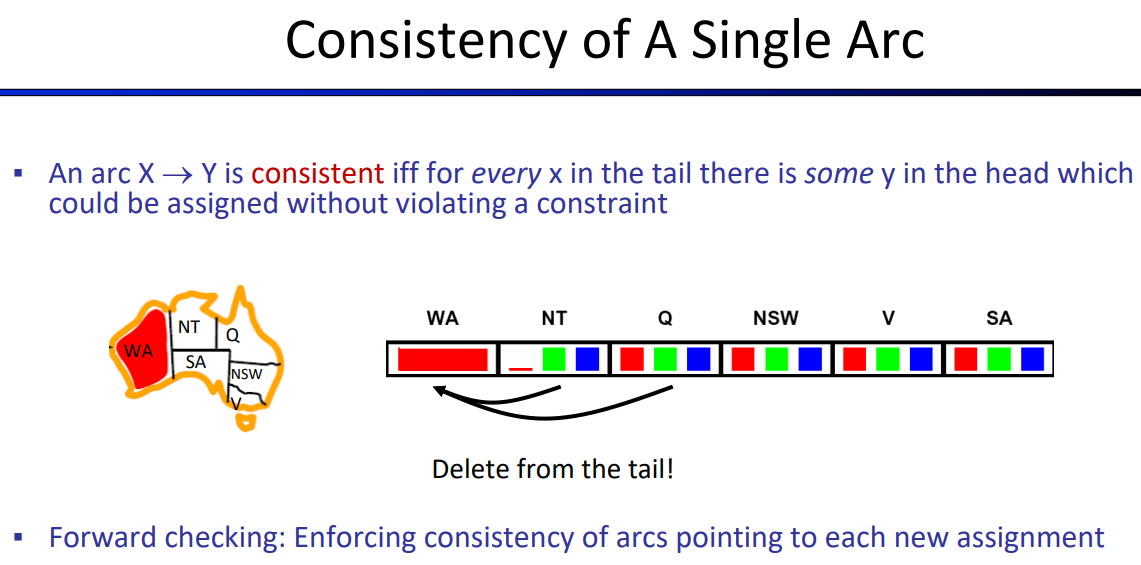
\includegraphics[width=\linewidth]{arc-consistency}
\end{figure}